% board-warping-lenses/bw_si_tamron.tex — generated by experiments/src/paper_figures/board_warping_offsets.jl; do not edit.
% One 3-D panel: the planar board of set bw_si_tamron (1000 x 1000 mm; x to the right, y up the page, z towards the camera) PLUS the offset
% vector that the lens's calibration gives every point (spline camera, refine product 2ddf016ec88be607): in the plane the print
% error Aspect(a = -5.45202e-05) o Skew(u = 0.000409712), along the normal the height. The whole vector is drawn 50 times as large as lengths on
% the page: the point of the page at (x, y) mm is at (x + 50 dx, y + 50 dy), its z is the height in mm. 5 x 5 mesh points; every
% patch has the colour of its height's band (0.5 mm); the dots are the warping's 5 x 5 nodes, displaced the same way.
% The picture is the orthographic view from azimuth 20, elevation 25 degrees with the heights 50 times as large as lengths on the
% page: PGFPlots stretches the projected unit cube of the axis ranges to width x height, which is that view when the x and y
% ranges are equal, `view`'s elevation is atan(range tan 25 / (50 * height range)) = 60.7758 degrees and height / width is the
% projection's. The box: the page widened by 75 mm (1.5 mm of offset) at all four sides, -3 ... +3 mm; the same margin and
% heights in every panel. Its width is \rcpanelwidth, of which 12 pt at the left hold the tick labels and their unit.
\providecommand{\rcfigdir}{src/fig}%
\providecommand{\rcpanelwidth}{\linewidth}%
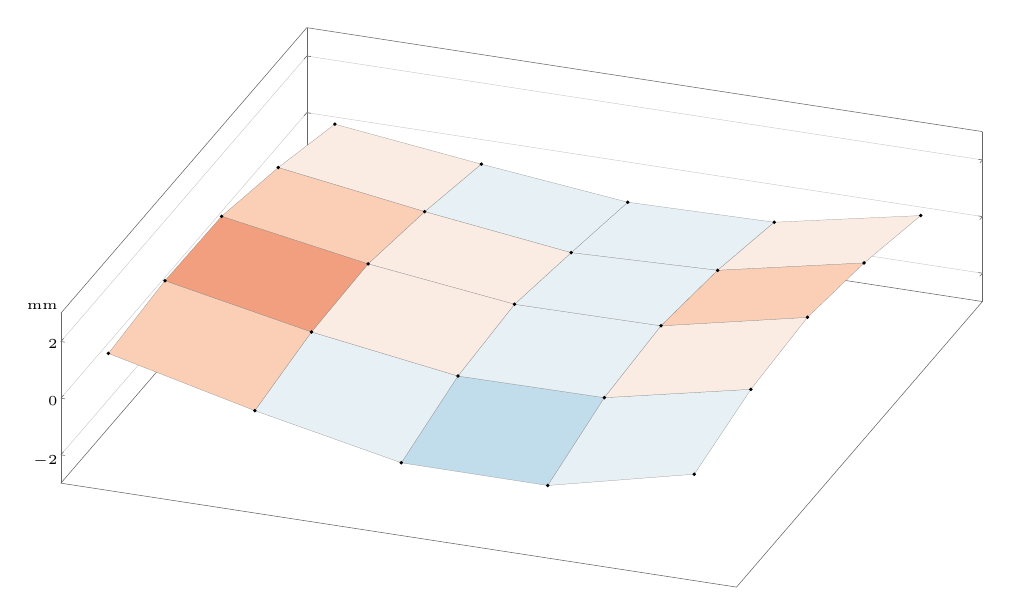
\begin{tikzpicture}[baseline=(current axis.center)]
\pgfmathsetlengthmacro{\rcwarpw}{\rcpanelwidth-12pt}%
\begin{axis}[
  scale only axis, width=\rcwarpw, height=0.60708*\rcwarpw, view={20}{60.7758},
  xmin=-75, xmax=1075.0, ymin=-75, ymax=1075.0, zmin=-3, zmax=3, clip=false,
  xtick=\empty, ytick=\empty, ztick={-2,0,2}, zticklabel style={font=\tiny, inner sep=1pt},
  tick style={line width=0.2pt, black!60}, major tick length=1.5pt, zmajorgrids, grid style={line width=0.15pt, black!22},
  axis line style={line width=0.2pt, black!60},
  colormap={warp}{rgb255=(17,70,128) rgb255=(42,113,178) rgb255=(74,151,197) rgb255=(139,193,220) rgb255=(193,221,236) rgb255=(231,240,244) rgb255=(250,235,227) rgb255=(251,206,182) rgb255=(241,159,126) rgb255=(217,102,81) rgb255=(187,42,52) rgb255=(134,10,36)}, colormap access=piecewise const, point meta min=-3, point meta max=3]
\addplot3[surf, shader=faceted, faceted color=black!45, line width=0.08pt, mesh/rows=5, z buffer=sort, point meta=z] coordinates {
(-20.48,-2.73,1.121) (228.83,-2.73,-0.104) (478.15,-2.73,-1.149) (727.47,-2.73,-1.155) (976.79,-2.73,0.038)
(-15.36,247.96,1.508) (233.96,247.96,0.494) (483.27,247.96,-0.267) (732.59,247.96,-0.235) (981.91,247.96,0.855)
(-10.24,498.64,1.599) (239.08,498.64,0.715) (488.39,498.64,0.085) (737.71,498.64,0.120) (987.03,498.64,1.214)
(-5.12,749.32,1.139) (244.20,749.32,0.378) (493.52,749.32,-0.275) (742.83,749.32,-0.103) (992.15,749.32,0.952)
(0.00,1000.00,0.490) (249.32,1000.00,-0.125) (498.64,1000.00,-0.674) (747.96,1000.00,-0.585) (997.27,1000.00,0.445)
};
\addplot3[only marks, mark=*, mark size=0.4pt, black] coordinates {(0.00,1000.00,0.490) (249.32,1000.00,-0.125) (498.64,1000.00,-0.674) (747.96,1000.00,-0.585) (997.27,1000.00,0.445) (-5.12,749.32,1.139) (244.20,749.32,0.378) (493.52,749.32,-0.275) (742.83,749.32,-0.103) (992.15,749.32,0.952) (-10.24,498.64,1.599) (239.08,498.64,0.715) (488.39,498.64,0.085) (737.71,498.64,0.120) (987.03,498.64,1.214) (-15.36,247.96,1.508) (233.96,247.96,0.494) (483.27,247.96,-0.267) (732.59,247.96,-0.235) (981.91,247.96,0.855) (-20.48,-2.73,1.121) (228.83,-2.73,-0.104) (478.15,-2.73,-1.149) (727.47,-2.73,-1.155) (976.79,-2.73,0.038)};
\node[anchor=south east, font=\tiny, inner sep=1pt] at (axis cs:-75,-75,3) {mm};   % the unit of the height's ticks, over their labels
\end{axis}
\pgfresetboundingbox\path ([xshift=-12pt]current axis.south west) rectangle (current axis.north east);   % the box is the axis and the strip of the tick labels
\end{tikzpicture}%
